\documentclass[a4paper]{article}
\usepackage[utf8]{inputenc}
\usepackage{amsmath}
\usepackage{amssymb}
\usepackage{siunitx}
\usepackage[ngerman]{babel}
\usepackage{pgfplots}
\usepackage{hyperref}
\usepackage{pgfplotstable}
\usepackage[section]{placeins}
\usepackage{enumitem}
\usepackage{float}
\usepackage{booktabs}
\usepackage[normalem]{ulem}
\usepackage{subcaption}
\usepackage{chngpage}
\usepackage[overload]{empheq}
\usepackage{todonotes}

\pgfplotsset{compat=1.15}

% Full Reference, produces: "Abbildung 3: Schaltplan"
\newcommand*{\fullref}[1]{\hyperref[{#1}]{\autoref*{#1}: \nameref*{#1}}}

\newcommand{\ugs}{U_{GS}}
\newcommand{\uds}{U_{DS}}
\newcommand{\uth}{U_{TH}}

\title{GPET\\ Auswertung Versuch 9\\ Gruppe 1}

\author{Jonas Otto\\ \href{mailto:jonas@jonasotto.com}{jonas@jonasotto.com} 
   \and Luca Krüger \\ \href{mailto:luca.krueger@uni-ulm.de}{luca.krueger@uni-ulm.de} }
\date{vom 12. Juni 2018}

\begin{document}

\maketitle

\newpage

\section{Vorbereitende Aufgaben und Fragen}

\subsection{Allgemeine Fragen}
\paragraph{1}
Wenn $U_{GS} \geq U_{TH}$ entsteht zwischen Source und Drain ein Kanal aus Elektronen als Ladungsträger, sodass Strom fließen kann.

\paragraph{2}
Beim Transistor gibt es folgende Arbeitsbereiche:
\begin{itemize}
    \item Sperrbereich: $\ugs < U_{TH}$, es kann kein Strom durch den Transistor fließen.
    \item Linearbereich: $\ugs \geq \uth$ und $(\ugs + \uth) > \uds$, Strom kann durch den Transistor fließen, bei $\uds \approx 0$ annähernd lineare Kennline
    \item Sättigungs- /Abschnürbereich: $\ugs \geq \uth$ und $\uds > (\ugs - \uth)$, Strom ist nahezu konstant (nicht von $\uds$ abhängig), Transistor gleicht einer durch $\ugs$ gesteuerten Stromquelle.
\end{itemize}


\paragraph{4}
In der Sättigung fließt ein konstanter Strom durch den Transistor. 

\paragraph{5} Es wird zwischen folgenden Arten von Gegenkopplung unterschieden:

\begin{itemize}
    \item VGK: Spannungsgegenkopplung, Teil der Ausgangsspannung wird zurückgeführt, Gegenkopplung verschwindet bei Kurzschluss des Ausgangs.
    \item AGK: Stromgegenkopplung, Teil des Ausgangsstzroms wird zurückgeführt, Gegenkopplung verschwindet bei Leerlauf des Ausgangs. 
\end{itemize}

\paragraph{6}
Da kein Strom $I_{GS}$ fließen muss, sondern im inneren des MOSFETs nur ein E-Feld aufgebaut werden muss. Sobald dieses besteht, fließt kein Strom mehr.

\subsection{Verstärker}
\paragraph{1}
Es wird ein selbstsperrender n-MOSFET verwendet.

\paragraph{2}
Für $Y_{DS}$ ist das Ausgangskennlinenfeld $I_D(\uds)$ relevant. $Y_{DS}$ beschreibt hier die Steigung des Graphen und stellt die Admittanz des Mosfets dar.

\paragraph{3}
Dieser Verstärker entspricht der \glqq Common-Source\grqq\ Schaltung.

\paragraph{4}
Die Kondensatoren stellen einen Hochpass dar und können so bei hoher Frequenz als Kurzschluss betrachtet werden.

\paragraph{5}
$Z_C=\frac{1}{j\omega C}=-72.3\cdot j \si{\ohm}$

\subsection{Class-A-Endstufe}
\paragraph{1}
Es handelt sich um eine \glqq Common-Drain\grqq\ Schaltung.

\paragraph{2}
Die Gegenkopplung ist eine Spannungsgegenkopplung, da $U_{R_L}=U_2$, und die steuernde Spannung $\ugs$ abhängig von $U_{R_L}$ ist: $\ugs = U_G - U_{R_L}$.

\paragraph{3}
Der Ausgangsstrom kann groß sein, was aber keinen Einfluss auf die Impedanz des Eingangs hat.


\section{Versuchsauswertung}

\subsection{Messung der Kennlinienfelder}
In diesem Versuch wurden die Kennlinien von zwei FETs mit den Bezeichnungen $T_1$(BS270) und $T_2$(IPP60R950C6) ermittelt.
Dazu wurden die beiden Transistoren wie in Abbildung \ref{fig:versuch1-aufbau} angeschlossen.

\begin{figure}[H]
    \centering
    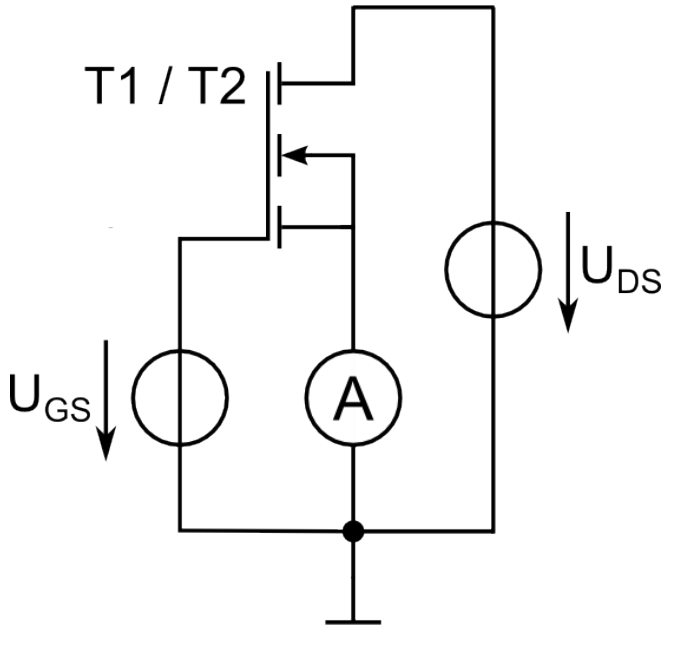
\includegraphics[width=5cm]{versuch1/versuch1_aufbau.png}
    \caption{Messaufbau zur Charakterisierung der FETs}
    \label{fig:versuch1-aufbau}
\end{figure}

Für die Gate-Source-Kennlinie von $T_$1 wird eine konstante Drain-Source-Spannung $\uds=3\si{V}V$ eingestellt.
\begin{figure}[H]
    \centering
        \begin{tikzpicture}
            \begin{axis}[
            xlabel={$\ugs [V]$},
            ylabel={$I_D [A]$}]
                \addplot table [x=u, y=I, col sep=comma, mark=none] {versuch1/versuch1_t1GS.csv};
            \end{axis}
        \end{tikzpicture}
    \caption{Kennlinie von $T_1$ bei $\uds$ konstant}
    \label{fig:kennlinie-t1-ugs}
\end{figure}

Für die Gate-Source-Kennlinie von $T_2$ wird eine konstante Drain-Source-Spannung $\uds=4\si{V}V$ eingestellt.
\begin{figure}[H]
    \centering
        \begin{tikzpicture}
            \begin{axis}[
            xlabel={$\ugs [V]$},
            ylabel={$I_D [A]$}]
                \addplot table [x=u, y=I, col sep=comma, mark=none] {versuch1/versuch1_t2GS.csv};
            \end{axis}
        \end{tikzpicture}
    \caption{Kennlinie von $T_2$ bei $\uds$ konstant}
    \label{fig:kennlinie-t2-ugs}
\end{figure}



Die Thresholdspannung $\uth$ der beiden Transistoren kann aus den Kennlinien für $\uds = \text{const}$ (Abbildung \ref{fig:kennlinie-t1-ugs}, \ref{fig:kennlinie-t2-ugs}) abgelesen werden: $\uth_1=2.5\si{V}$, $\uth_2=3.6\si{V}$. Die Steilheit des Transistors T1 beträgt $S=\frac{I}{U}= 0.067\frac{A}{V}$.

Für die Drain-Source-Kennlinie von $T_1$ wird eine konstante Gate-Source-Spannung von $\ugs=3\si{V}$ eingestellt.
\begin{figure}[H]
    \centering
        \begin{tikzpicture}
            \begin{axis}[
            xlabel={$\uds [V]$},
            ylabel={$I_D [A]$}]
                \addplot table [x=u, y=I, col sep=comma, mark=none] {versuch1/versuch1_t1DS.csv};
            \end{axis}
        \end{tikzpicture}
    \caption{Kennlinie von $T_1$ bei $\ugs$ konstant}
    \label{fig:kennlinie-t1-uds}
\end{figure}
Für die Drain-Source-Kennlinie von $T_2$ wird eine konstante Gate-Source-Spannung von $\ugs=4\si{V}$ eingestellt.
\begin{figure}[H]
    \centering
        \begin{tikzpicture}
            \begin{axis}[
            xlabel={$\uds [V]$},
            ylabel={$I_D [A]$}]
                \addplot table [x=u, y=I, col sep=comma, mark=none] {versuch1/versuch1_t2DS.csv};
            \end{axis}
        \end{tikzpicture}
    \caption{Kennlinie von $T_2$ bei $\ugs$ konstant}
    \label{fig:kennlinie-t2-uds}
\end{figure}

Der Widerstand $R_{DS}$ von $T_1$ beträgt $60\si{\ohm}$, was dem inversen der Steigung der Kennline in Abbildung \ref{fig:kennlinie-t1-uds} entspricht.

\subsection{Verstärker}

\begin{figure}[H]
    \centering
    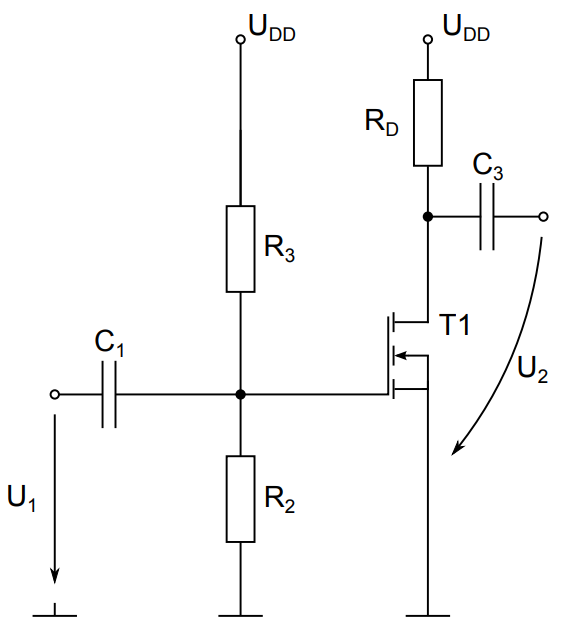
\includegraphics[width=0.7\textwidth]{versuch2/versuch2_aufbau.png}
    \caption{Verstärkernetzwerk}
    \label{fig:versuch2-aufbau}
\end{figure}

In diesem Versuch wurde mit einem FET eine Verstärkerschaltung(Abbildung \ref{fig:versuch2-aufbau}) realisiert, die keine Gegenkopplung besitzt und mit Wechselspannung unterschiedlicher Frequenzen betrieben wurde.

\paragraph{Messung des Amplitudengangs}
Im folgenden wurde die Frequenzabhängigkeit der Verstärkung gemessen.

\begin{figure}[H]
    \centering
        \begin{tikzpicture}
            \begin{axis}[
            xlabel={$f [\si{Hz}]$},
            ylabel={$A_V [\si{dB}]$},
            xmode=log]
                \addplot[color=red,mark=x] coordinates {
            		(100,39)            %100    9
            		(500,40.6)          %500    10.7
            		(1000,40)           %1k     10.1
            		(5000,40)           %5k     10.1
            		(10000,40.25)       %10k    10.3
            		(50000,40)          %50k    10.1
            		(100000,40)         %100k   10.1
            		(500000,41.2)       %500k   11.5
            		(1000000,38)        %1M     8
            		(4000000,30.57)     %4M     3.38
            		};
            \end{axis}
        \end{tikzpicture}
    \caption{Amplitudengang}
    \label{fig:verstaerker-amplitude}
\end{figure}

In Abbildung \ref{fig:verstaerker-amplitude} ist die frequenzabhängige Amplitude zu sehen. Aufgrund von Störungen im Signal und einem Steckbrett, das keine zuverlässige Verbindung zwischen den Bauteilen sicherstellen konnte, konnte kein Plot mit MatLab angefertigt werden. Der manuell aufgenommene Plot zeigt, dass die Verstärkung bei hohen Frequenzen zwar abnimmt, aber im Bereich von $500\si{Hz}$ bis $500\si{kHz}$ relativ konstant bei $\approx 40\si{dB}$ liegt. Die Verstärkung bei $f=1\si{kHz}$ beträgt $\approx 40 \si{dB}$.

Die Bandbreite kann mit unserem Plot leider nicht bestimmt werden, eigentlich sollte der Plot wie in Abbildung \ref{fig:verstaerker-amplitude-ideal} aussehen, was einer Bandbreite von $100\si{Hz}$ bis $1\si{MHz}$ entspricht.

\begin{figure}[H]
    \centering
    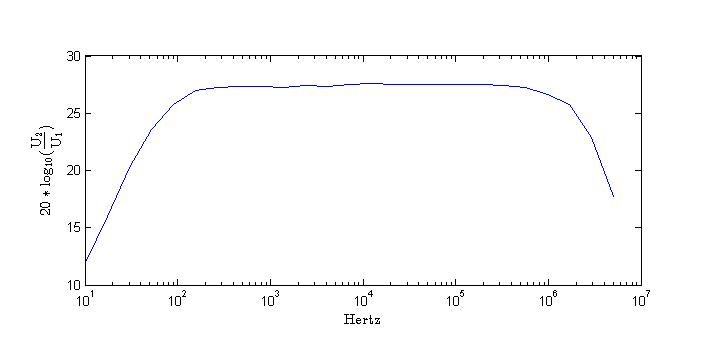
\includegraphics[width=0.8\textwidth]{versuch3/4_3_Amplitudengang_01.jpg}
    \caption{Frequenzabhängigkeit der Amplitude}
    \label{fig:verstaerker-amplitude-ideal}
\end{figure}

\subsection{Class-A Endstufe}
In diesem Versuch wurde eine Class-A Endstufe aufgebaut und später hinter den Verstärker geschaltet. Diese wurde wieder mit Wechselspannung betrieben.
\begin{figure}[H]
    \centering
    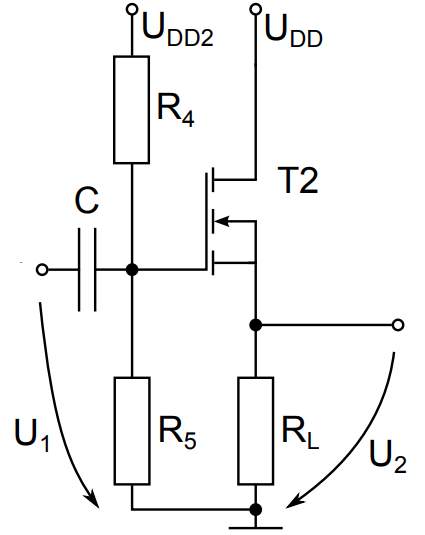
\includegraphics[width=0.5\textwidth]{versuch3/versuch3_aufbau.png}
    \caption{Class-A Endstufe}
    \label{fig:versuch3-aufbau}
\end{figure}

Wie in Abbildung \ref{fig:versuch3-verstaerkung} zu erkennen, beträgt die Verstärkung $\frac{U_2}{U_1}=\frac{2.92}{0.49}=5.9$. Dabei wird allerdings nicht die Peak-Peak Spannung erhöht, sondern nur ein Gleichanteil von $\approx 2.5\si{V}$ hinzugefügt.


\begin{figure}[H]
    \centering
    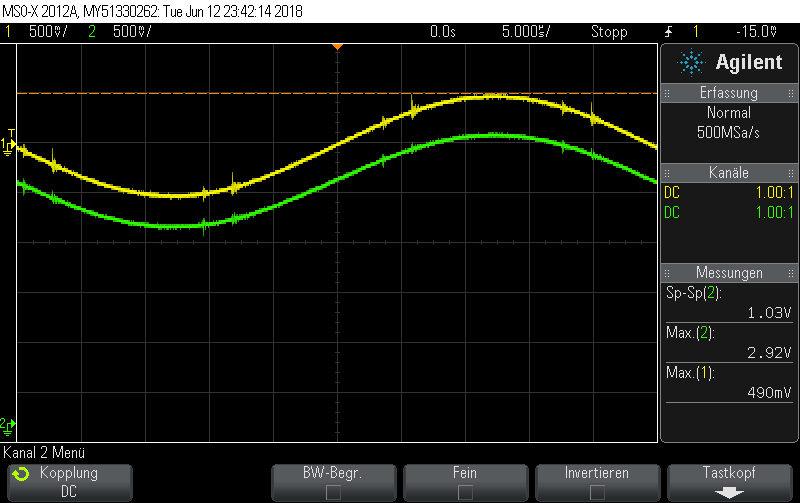
\includegraphics[width=0.8\textwidth]{versuch3/versuch3_endstufe.png}
    \caption{Verstärkung der Class-A-Endstufe}
    \label{fig:versuch3-verstaerkung}
\end{figure}


Wenn die Class-A Endstufe nach dem Verstärker aus dem vorherigen Versuch geschaltet wird, kann wie erwartet der Kopfhörer betrieben werden. Die Frequenzen werden verstärkt, wie in Abbildung \ref{fig:versuch3-audio} zu sehen ist.

\begin{figure}[H]
    \centering
    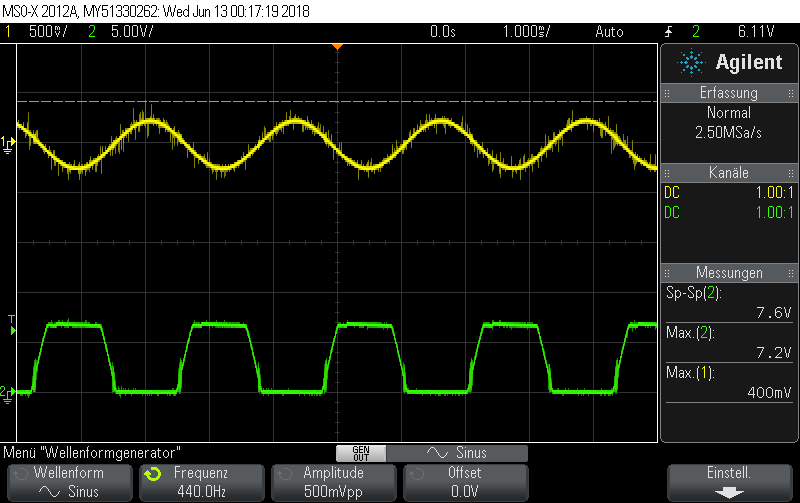
\includegraphics[width=0.8\textwidth]{versuch3/versuch3_audio.png}
    \caption{Vollständiger Signalpfad, Verstärker mit Endstufe}
    \label{fig:versuch3-audio}
\end{figure}

\end{document}
